\documentclass[twoside]{book}

% Packages required by doxygen
\usepackage{fixltx2e}
\usepackage{calc}
\usepackage{doxygen}
\usepackage[export]{adjustbox} % also loads graphicx
\usepackage{graphicx}
\usepackage[utf8]{inputenc}
\usepackage{makeidx}
\usepackage{multicol}
\usepackage{multirow}
\PassOptionsToPackage{warn}{textcomp}
\usepackage{textcomp}
\usepackage[nointegrals]{wasysym}
\usepackage[table]{xcolor}

% Font selection
\usepackage[T1]{fontenc}
\usepackage[scaled=.90]{helvet}
\usepackage{courier}
\usepackage{amssymb}
\usepackage{sectsty}
\renewcommand{\familydefault}{\sfdefault}
\allsectionsfont{%
  \fontseries{bc}\selectfont%
  \color{darkgray}%
}
\renewcommand{\DoxyLabelFont}{%
  \fontseries{bc}\selectfont%
  \color{darkgray}%
}
\newcommand{\+}{\discretionary{\mbox{\scriptsize$\hookleftarrow$}}{}{}}

% Page & text layout
\usepackage{geometry}
\geometry{%
  a4paper,%
  top=2.5cm,%
  bottom=2.5cm,%
  left=2.5cm,%
  right=2.5cm%
}
\tolerance=750
\hfuzz=15pt
\hbadness=750
\setlength{\emergencystretch}{15pt}
\setlength{\parindent}{0cm}
\setlength{\parskip}{3ex plus 2ex minus 2ex}
\makeatletter
\renewcommand{\paragraph}{%
  \@startsection{paragraph}{4}{0ex}{-1.0ex}{1.0ex}{%
    \normalfont\normalsize\bfseries\SS@parafont%
  }%
}
\renewcommand{\subparagraph}{%
  \@startsection{subparagraph}{5}{0ex}{-1.0ex}{1.0ex}{%
    \normalfont\normalsize\bfseries\SS@subparafont%
  }%
}
\makeatother

% Headers & footers
\usepackage{fancyhdr}
\pagestyle{fancyplain}
\fancyhead[LE]{\fancyplain{}{\bfseries\thepage}}
\fancyhead[CE]{\fancyplain{}{}}
\fancyhead[RE]{\fancyplain{}{\bfseries\leftmark}}
\fancyhead[LO]{\fancyplain{}{\bfseries\rightmark}}
\fancyhead[CO]{\fancyplain{}{}}
\fancyhead[RO]{\fancyplain{}{\bfseries\thepage}}
\fancyfoot[LE]{\fancyplain{}{}}
\fancyfoot[CE]{\fancyplain{}{}}
\fancyfoot[RE]{\fancyplain{}{\bfseries\scriptsize Generated by Doxygen }}
\fancyfoot[LO]{\fancyplain{}{\bfseries\scriptsize Generated by Doxygen }}
\fancyfoot[CO]{\fancyplain{}{}}
\fancyfoot[RO]{\fancyplain{}{}}
\renewcommand{\footrulewidth}{0.4pt}
\renewcommand{\chaptermark}[1]{%
  \markboth{#1}{}%
}
\renewcommand{\sectionmark}[1]{%
  \markright{\thesection\ #1}%
}

% Indices & bibliography
\usepackage{natbib}
\usepackage[titles]{tocloft}
\setcounter{tocdepth}{3}
\setcounter{secnumdepth}{5}
\makeindex

% Hyperlinks (required, but should be loaded last)
\usepackage{ifpdf}
\ifpdf
  \usepackage[pdftex,pagebackref=true]{hyperref}
\else
  \usepackage[ps2pdf,pagebackref=true]{hyperref}
\fi
\hypersetup{%
  colorlinks=true,%
  linkcolor=blue,%
  citecolor=blue,%
  unicode%
}

% Custom commands
\newcommand{\clearemptydoublepage}{%
  \newpage{\pagestyle{empty}\cleardoublepage}%
}

\usepackage{caption}
\captionsetup{labelsep=space,justification=centering,font={bf},singlelinecheck=off,skip=4pt,position=top}

%===== C O N T E N T S =====

\begin{document}

% Titlepage & ToC
\hypersetup{pageanchor=false,
             bookmarksnumbered=true,
             pdfencoding=unicode
            }
\pagenumbering{roman}
\begin{titlepage}
\vspace*{7cm}
\begin{center}%
{\Large My Project }\\
\vspace*{1cm}
{\large Generated by Doxygen 1.8.11}\\
\end{center}
\end{titlepage}
\clearemptydoublepage
\tableofcontents
\clearemptydoublepage
\pagenumbering{arabic}
\hypersetup{pageanchor=true}

%--- Begin generated contents ---
\chapter{Class Index}
\section{Class List}
Here are the classes, structs, unions and interfaces with brief descriptions\+:\begin{DoxyCompactList}
\item\contentsline{section}{\hyperlink{structnode}{node} }{\pageref{structnode}}{}
\item\contentsline{section}{\hyperlink{structnode1}{node1} }{\pageref{structnode1}}{}
\item\contentsline{section}{\hyperlink{structnode__info}{node\+\_\+info} }{\pageref{structnode__info}}{}
\end{DoxyCompactList}

\chapter{File Index}
\section{File List}
Here is a list of all files with brief descriptions\+:\begin{DoxyCompactList}
\item\contentsline{section}{\hyperlink{Lab1_8c}{Lab1.\+c} }{\pageref{Lab1_8c}}{}
\end{DoxyCompactList}

\chapter{Class Documentation}
\hypertarget{classPriorityLock}{}\section{Priority\+Lock Class Reference}
\label{classPriorityLock}\index{Priority\+Lock@{Priority\+Lock}}
\subsection*{Public Member Functions}
\begin{DoxyCompactItemize}
\item 
void \hyperlink{classPriorityLock_a8891b1ac7ee3de2ff39a0dd1791349fb}{enter} (int priority\+\_\+level)
\item 
void \hyperlink{classPriorityLock_a572356166105b668acfebe6549da71d2}{exit} ()
\item 
\hyperlink{classPriorityLock_a88083d767c98de77f22cd9243304652d}{Priority\+Lock} ()
\end{DoxyCompactItemize}
\subsection*{Private Attributes}
\begin{DoxyCompactItemize}
\item 
priority\+\_\+queue$<$ int $>$ \hyperlink{classPriorityLock_ae1c22f9c1af23bfdc5db44bf52888c32}{wait\+\_\+list}
\item 
pthread\+\_\+mutex\+\_\+t \hyperlink{classPriorityLock_ae9ab1ff618b71f318e9cd7b8407f44c0}{lock}
\item 
pthread\+\_\+cond\+\_\+t \hyperlink{classPriorityLock_ab79a742b197e6d569299a77234590ebd}{pop\+Top}
\end{DoxyCompactItemize}


\subsection{Constructor \& Destructor Documentation}
\index{Priority\+Lock@{Priority\+Lock}!Priority\+Lock@{Priority\+Lock}}
\index{Priority\+Lock@{Priority\+Lock}!Priority\+Lock@{Priority\+Lock}}
\subsubsection[{\texorpdfstring{Priority\+Lock()}{PriorityLock()}}]{\setlength{\rightskip}{0pt plus 5cm}Priority\+Lock\+::\+Priority\+Lock (
\begin{DoxyParamCaption}
{}
\end{DoxyParamCaption}
)}\hypertarget{classPriorityLock_a88083d767c98de77f22cd9243304652d}{}\label{classPriorityLock_a88083d767c98de77f22cd9243304652d}

\begin{DoxyCode}
42 \{
43    \textcolor{comment}{//initialize variables                                                                                  
                                                                                                       }
44    \hyperlink{classPriorityLock_ae9ab1ff618b71f318e9cd7b8407f44c0}{lock} = PTHREAD\_MUTEX\_INITIALIZER;
45    \hyperlink{classPriorityLock_ab79a742b197e6d569299a77234590ebd}{popTop} = PTHREAD\_COND\_INITIALIZER;
46 \}
\end{DoxyCode}


\subsection{Member Function Documentation}
\index{Priority\+Lock@{Priority\+Lock}!enter@{enter}}
\index{enter@{enter}!Priority\+Lock@{Priority\+Lock}}
\subsubsection[{\texorpdfstring{enter(int priority\+\_\+level)}{enter(int priority_level)}}]{\setlength{\rightskip}{0pt plus 5cm}void Priority\+Lock\+::enter (
\begin{DoxyParamCaption}
\item[{int}]{priority\+\_\+level}
\end{DoxyParamCaption}
)}\hypertarget{classPriorityLock_a8891b1ac7ee3de2ff39a0dd1791349fb}{}\label{classPriorityLock_a8891b1ac7ee3de2ff39a0dd1791349fb}

\begin{DoxyCode}
49 \{
50    pthread\_mutex\_lock(&\hyperlink{classPriorityLock_ae9ab1ff618b71f318e9cd7b8407f44c0}{lock});
51    \hyperlink{classPriorityLock_ae1c22f9c1af23bfdc5db44bf52888c32}{wait\_list}.push(priority\_level);
52    \textcolor{keywordflow}{while}(\hyperlink{classPriorityLock_ae1c22f9c1af23bfdc5db44bf52888c32}{wait\_list}.top() != priority\_level)\{
53       pthread\_cond\_wait(&\hyperlink{classPriorityLock_ab79a742b197e6d569299a77234590ebd}{popTop}, &\hyperlink{classPriorityLock_ae9ab1ff618b71f318e9cd7b8407f44c0}{lock});
54    \}
55    cout << \textcolor{stringliteral}{"Length of priority queue: "} << \hyperlink{classPriorityLock_ae1c22f9c1af23bfdc5db44bf52888c32}{wait\_list}.size() << endl;
56    pthread\_mutex\_unlock(&\hyperlink{classPriorityLock_ae9ab1ff618b71f318e9cd7b8407f44c0}{lock});
57 \}
\end{DoxyCode}
\index{Priority\+Lock@{Priority\+Lock}!exit@{exit}}
\index{exit@{exit}!Priority\+Lock@{Priority\+Lock}}
\subsubsection[{\texorpdfstring{exit()}{exit()}}]{\setlength{\rightskip}{0pt plus 5cm}void Priority\+Lock\+::exit (
\begin{DoxyParamCaption}
{}
\end{DoxyParamCaption}
)}\hypertarget{classPriorityLock_a572356166105b668acfebe6549da71d2}{}\label{classPriorityLock_a572356166105b668acfebe6549da71d2}

\begin{DoxyCode}
60 \{
61    pthread\_mutex\_lock(&\hyperlink{classPriorityLock_ae9ab1ff618b71f318e9cd7b8407f44c0}{lock});
62    \hyperlink{classPriorityLock_ae1c22f9c1af23bfdc5db44bf52888c32}{wait\_list}.pop();
63    pthread\_cond\_broadcast(&\hyperlink{classPriorityLock_ab79a742b197e6d569299a77234590ebd}{popTop});
64    pthread\_mutex\_unlock(&\hyperlink{classPriorityLock_ae9ab1ff618b71f318e9cd7b8407f44c0}{lock});
65 \}
\end{DoxyCode}


\subsection{Member Data Documentation}
\index{Priority\+Lock@{Priority\+Lock}!lock@{lock}}
\index{lock@{lock}!Priority\+Lock@{Priority\+Lock}}
\subsubsection[{\texorpdfstring{lock}{lock}}]{\setlength{\rightskip}{0pt plus 5cm}pthread\+\_\+mutex\+\_\+t Priority\+Lock\+::lock\hspace{0.3cm}{\ttfamily [private]}}\hypertarget{classPriorityLock_ae9ab1ff618b71f318e9cd7b8407f44c0}{}\label{classPriorityLock_ae9ab1ff618b71f318e9cd7b8407f44c0}
\index{Priority\+Lock@{Priority\+Lock}!pop\+Top@{pop\+Top}}
\index{pop\+Top@{pop\+Top}!Priority\+Lock@{Priority\+Lock}}
\subsubsection[{\texorpdfstring{pop\+Top}{popTop}}]{\setlength{\rightskip}{0pt plus 5cm}pthread\+\_\+cond\+\_\+t Priority\+Lock\+::pop\+Top\hspace{0.3cm}{\ttfamily [private]}}\hypertarget{classPriorityLock_ab79a742b197e6d569299a77234590ebd}{}\label{classPriorityLock_ab79a742b197e6d569299a77234590ebd}
\index{Priority\+Lock@{Priority\+Lock}!wait\+\_\+list@{wait\+\_\+list}}
\index{wait\+\_\+list@{wait\+\_\+list}!Priority\+Lock@{Priority\+Lock}}
\subsubsection[{\texorpdfstring{wait\+\_\+list}{wait_list}}]{\setlength{\rightskip}{0pt plus 5cm}priority\+\_\+queue$<$int$>$ Priority\+Lock\+::wait\+\_\+list\hspace{0.3cm}{\ttfamily [private]}}\hypertarget{classPriorityLock_ae1c22f9c1af23bfdc5db44bf52888c32}{}\label{classPriorityLock_ae1c22f9c1af23bfdc5db44bf52888c32}


The documentation for this class was generated from the following file\+:\begin{DoxyCompactItemize}
\item 
\hyperlink{Lab4_8cpp}{Lab4.\+cpp}\end{DoxyCompactItemize}

\hypertarget{structThreadParam}{}\section{Thread\+Param Struct Reference}
\label{structThreadParam}\index{Thread\+Param@{Thread\+Param}}
\subsection*{Public Attributes}
\begin{DoxyCompactItemize}
\item 
int $\ast$ \hyperlink{structThreadParam_aec444b4eb12a9a8fea3e8689e149c222}{array}
\item 
int \hyperlink{structThreadParam_a67d5841b5ec120d0265bc55eeb8bac6b}{value}
\item 
int \hyperlink{structThreadParam_a48b6fa880b0369abac96f8f54bf12e08}{start\+Index}
\item 
int \hyperlink{structThreadParam_a88bf854942e7037fbdd9269b434612d6}{end\+Index}
\end{DoxyCompactItemize}


\subsection{Member Data Documentation}
\index{Thread\+Param@{Thread\+Param}!array@{array}}
\index{array@{array}!Thread\+Param@{Thread\+Param}}
\subsubsection[{\texorpdfstring{array}{array}}]{\setlength{\rightskip}{0pt plus 5cm}int$\ast$ Thread\+Param\+::array}\hypertarget{structThreadParam_aec444b4eb12a9a8fea3e8689e149c222}{}\label{structThreadParam_aec444b4eb12a9a8fea3e8689e149c222}
\index{Thread\+Param@{Thread\+Param}!end\+Index@{end\+Index}}
\index{end\+Index@{end\+Index}!Thread\+Param@{Thread\+Param}}
\subsubsection[{\texorpdfstring{end\+Index}{endIndex}}]{\setlength{\rightskip}{0pt plus 5cm}int Thread\+Param\+::end\+Index}\hypertarget{structThreadParam_a88bf854942e7037fbdd9269b434612d6}{}\label{structThreadParam_a88bf854942e7037fbdd9269b434612d6}
\index{Thread\+Param@{Thread\+Param}!start\+Index@{start\+Index}}
\index{start\+Index@{start\+Index}!Thread\+Param@{Thread\+Param}}
\subsubsection[{\texorpdfstring{start\+Index}{startIndex}}]{\setlength{\rightskip}{0pt plus 5cm}int Thread\+Param\+::start\+Index}\hypertarget{structThreadParam_a48b6fa880b0369abac96f8f54bf12e08}{}\label{structThreadParam_a48b6fa880b0369abac96f8f54bf12e08}
\index{Thread\+Param@{Thread\+Param}!value@{value}}
\index{value@{value}!Thread\+Param@{Thread\+Param}}
\subsubsection[{\texorpdfstring{value}{value}}]{\setlength{\rightskip}{0pt plus 5cm}int Thread\+Param\+::value}\hypertarget{structThreadParam_a67d5841b5ec120d0265bc55eeb8bac6b}{}\label{structThreadParam_a67d5841b5ec120d0265bc55eeb8bac6b}


The documentation for this struct was generated from the following file\+:\begin{DoxyCompactItemize}
\item 
\hyperlink{Lab3_8cpp}{Lab3.\+cpp}\end{DoxyCompactItemize}

\chapter{File Documentation}
\hypertarget{Lab4_8cpp}{}\section{Lab4.\+cpp File Reference}
\label{Lab4_8cpp}\index{Lab4.\+cpp@{Lab4.\+cpp}}
{\ttfamily \#include $<$iostream$>$}\\*
{\ttfamily \#include $<$pthread.\+h$>$}\\*
{\ttfamily \#include $<$stdio.\+h$>$}\\*
{\ttfamily \#include $<$stdlib.\+h$>$}\\*
{\ttfamily \#include $<$unistd.\+h$>$}\\*
{\ttfamily \#include $<$queue$>$}\\*
Include dependency graph for Lab4.\+cpp\+:
\nopagebreak
\begin{figure}[H]
\begin{center}
\leavevmode
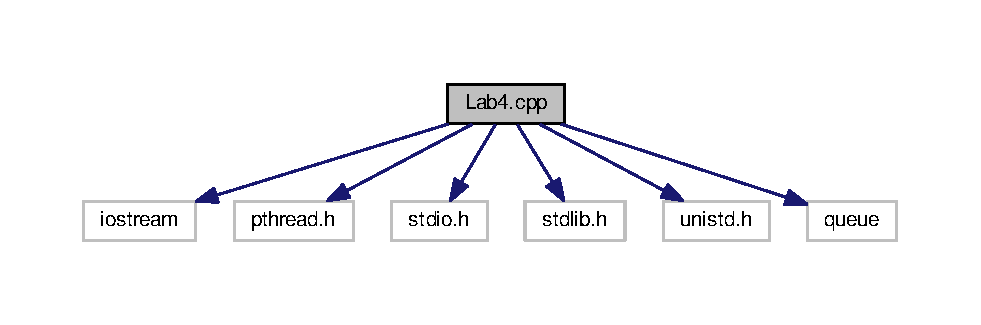
\includegraphics[width=350pt]{Lab4_8cpp__incl}
\end{center}
\end{figure}
\subsection*{Classes}
\begin{DoxyCompactItemize}
\item 
struct \hyperlink{structThreadParam}{Thread\+Param}
\item 
class \hyperlink{classPriorityLock}{Priority\+Lock}
\end{DoxyCompactItemize}
\subsection*{Functions}
\begin{DoxyCompactItemize}
\item 
void $\ast$ \hyperlink{Lab4_8cpp_a649e5687563f66a85f560f736a993494}{Thread\+Routine} (void $\ast$param)
\item 
int \hyperlink{Lab4_8cpp_a0ddf1224851353fc92bfbff6f499fa97}{main} (int argc, char $\ast$argv\mbox{[}$\,$\mbox{]})
\end{DoxyCompactItemize}
\subsection*{Variables}
\begin{DoxyCompactItemize}
\item 
\hyperlink{classPriorityLock}{Priority\+Lock} \hyperlink{Lab4_8cpp_aed51fc48bbdfd4e9f1f3c8ec0ce7586a}{plock}
\end{DoxyCompactItemize}


\subsection{Function Documentation}
\index{Lab4.\+cpp@{Lab4.\+cpp}!main@{main}}
\index{main@{main}!Lab4.\+cpp@{Lab4.\+cpp}}
\subsubsection[{\texorpdfstring{main(int argc, char $\ast$argv[])}{main(int argc, char *argv[])}}]{\setlength{\rightskip}{0pt plus 5cm}int main (
\begin{DoxyParamCaption}
\item[{int}]{argc, }
\item[{char $\ast$}]{argv\mbox{[}$\,$\mbox{]}}
\end{DoxyParamCaption}
)}\hypertarget{Lab4_8cpp_a0ddf1224851353fc92bfbff6f499fa97}{}\label{Lab4_8cpp_a0ddf1224851353fc92bfbff6f499fa97}

\begin{DoxyCode}
85 \{
86    pthread\_t * threads;
87    \hyperlink{structThreadParam}{ThreadParam} * priorityParams;
88 
89    \textcolor{keywordtype}{int} thread\_num;
90    \textcolor{keywordtype}{int} status, i, j;
91 
92    \textcolor{keywordflow}{do} \{
93       cout <<\textcolor{stringliteral}{"How many threads to create:"};
94       cin >> thread\_num;
95    \} \textcolor{keywordflow}{while} (thread\_num<=1);
96 
97    threads = \textcolor{keyword}{new} pthread\_t[thread\_num]; \textcolor{comment}{//dynamically allocate the thread handler ...                      
                                                                                                       }
98 
99    priorityParams = \textcolor{keyword}{new} \hyperlink{structThreadParam}{ThreadParam}[thread\_num];
100 
101    \textcolor{keywordflow}{for} (i=0; i<thread\_num; i++)\{
102       \textcolor{comment}{//Todo: prepare the argument to be passed in thread                                                  
                                                                                                       }
103       \textcolor{comment}{//                                                                                                   
                                                                                                       }
104       priorityParams[i].\hyperlink{structThreadParam_af65f9da248fc152676a9e6040138515b}{level} = rand()%100;
105 
106       status = pthread\_create (&threads[i], NULL, \hyperlink{Lab4_8cpp_a649e5687563f66a85f560f736a993494}{ThreadRoutine}, (\textcolor{keywordtype}{void} *)&(priorityParams[i]))
      ;
107 
108       \textcolor{keywordflow}{if} (status!=0)\{
109          printf (\textcolor{stringliteral}{"oops, pthread\_create returned error code %d\(\backslash\)n"}, status);
110          exit(-1);
111       \}
112    \}
113 
114    \textcolor{comment}{//EZ: Important that we wait for all threads to finish before ending the main thread ...                
                                                                                                       }
115    \textcolor{keywordflow}{for} (i=0; i<thread\_num; i++)\{
116       pthread\_join (threads[i],NULL);
117    \}
118 \}
\end{DoxyCode}


Here is the call graph for this function\+:
\nopagebreak
\begin{figure}[H]
\begin{center}
\leavevmode
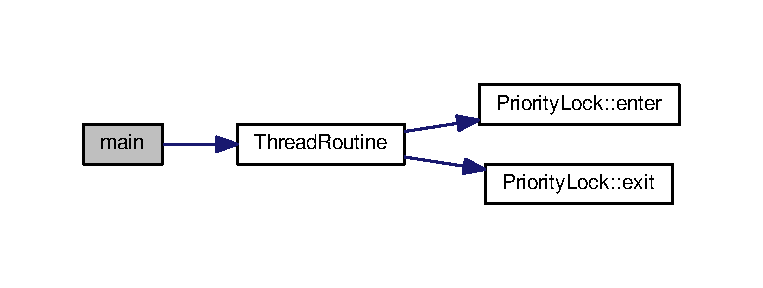
\includegraphics[width=350pt]{Lab4_8cpp_a0ddf1224851353fc92bfbff6f499fa97_cgraph}
\end{center}
\end{figure}


\index{Lab4.\+cpp@{Lab4.\+cpp}!Thread\+Routine@{Thread\+Routine}}
\index{Thread\+Routine@{Thread\+Routine}!Lab4.\+cpp@{Lab4.\+cpp}}
\subsubsection[{\texorpdfstring{Thread\+Routine(void $\ast$param)}{ThreadRoutine(void *param)}}]{\setlength{\rightskip}{0pt plus 5cm}void$\ast$ Thread\+Routine (
\begin{DoxyParamCaption}
\item[{void $\ast$}]{param}
\end{DoxyParamCaption}
)}\hypertarget{Lab4_8cpp_a649e5687563f66a85f560f736a993494}{}\label{Lab4_8cpp_a649e5687563f66a85f560f736a993494}

\begin{DoxyCode}
71 \{
72    \hyperlink{structThreadParam}{ThreadParam} * p = (\hyperlink{structThreadParam}{ThreadParam} *) param;
73    \textcolor{keywordtype}{int} priority\_level = p->\hyperlink{structThreadParam_af65f9da248fc152676a9e6040138515b}{level};
74 
75    cout <<\textcolor{stringliteral}{"Thread "}<< priority\_level << \textcolor{stringliteral}{" calling enter \(\backslash\)n"};
76    \hyperlink{Lab4_8cpp_aed51fc48bbdfd4e9f1f3c8ec0ce7586a}{plock}.\hyperlink{classPriorityLock_a8891b1ac7ee3de2ff39a0dd1791349fb}{enter} (priority\_level);
77 
78    cout <<\textcolor{stringliteral}{"Thread "}<< priority\_level << \textcolor{stringliteral}{" in critical section \(\backslash\)n"};
79 
80    \hyperlink{Lab4_8cpp_aed51fc48bbdfd4e9f1f3c8ec0ce7586a}{plock}.\hyperlink{classPriorityLock_a572356166105b668acfebe6549da71d2}{exit}();
81    cout << \textcolor{stringliteral}{"Thread "} << priority\_level << \textcolor{stringliteral}{" is done\(\backslash\)n"};
82 \}
\end{DoxyCode}


Here is the call graph for this function\+:
\nopagebreak
\begin{figure}[H]
\begin{center}
\leavevmode
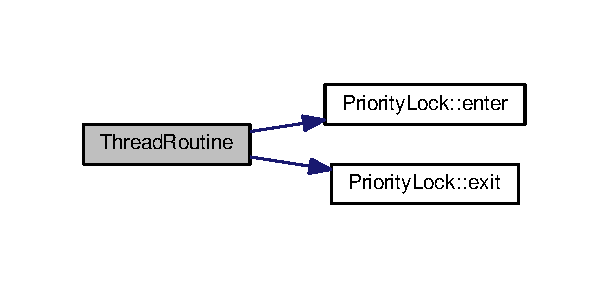
\includegraphics[width=292pt]{Lab4_8cpp_a649e5687563f66a85f560f736a993494_cgraph}
\end{center}
\end{figure}




\subsection{Variable Documentation}
\index{Lab4.\+cpp@{Lab4.\+cpp}!plock@{plock}}
\index{plock@{plock}!Lab4.\+cpp@{Lab4.\+cpp}}
\subsubsection[{\texorpdfstring{plock}{plock}}]{\setlength{\rightskip}{0pt plus 5cm}{\bf Priority\+Lock} plock}\hypertarget{Lab4_8cpp_aed51fc48bbdfd4e9f1f3c8ec0ce7586a}{}\label{Lab4_8cpp_aed51fc48bbdfd4e9f1f3c8ec0ce7586a}

%--- End generated contents ---

% Index
\backmatter
\newpage
\phantomsection
\clearemptydoublepage
\addcontentsline{toc}{chapter}{Index}
\printindex

\end{document}
